% !Mode:: "TeX:UTF-8"

\chapter{预备知识}
\label{ch:pre}



\section{图像的视觉信息抽取}



\subsection{卷积神经网络}

\subsubsection{卷积神经网络的介绍}
卷积神经网络(Convolutional Neural Network,CNN)是深度学习的代表算法之一,由LeCun首次实现并且应用。卷积神经网络的主要作用是提取特征,该网络收到生物学的影响,相比较与全连接神经网络,卷积神经网络的主要特性包括局部感知和参数共享。局部感知指对于具有空间特征的输入来说,每个神经元没必要知道全局的信息,只需要感知局部的信息,然后在更高层将局部的信息合并起来得到更高层的信息。对于权值共享来说,每个卷积核与位置无关,因为假设对于图像来说,其中某一部分的统计特性和其它的部分是一样的,所以对于其中的一个卷积核来说,可以应用到图像上的任何地方去。所以,局部感知和参数共享不仅能提取到更多的特征,并且能大幅度减少参数的数量。因此,卷积神经网络广泛的应用在图像、视频、音频和文本等各种模态的数据上,并且都取得了巨大的成功。

卷积神经网络的特征提取层主要包括两个模块,分别是卷积层(convolutional layer)和池化层(pooling layer),两者的顺序,一般是先通过卷积层,然后是池化层。对于卷积层,主要的作用是提取特征,卷积层的核心是卷积核(kernel),其本质还是神经元。但是卷积核的感受野和全连接的神经元是不同的,这里的感受野是局部的,并且感受野的大小由卷积核的大小控制。如图\ref{fig:con-example}所示,当前卷积核的大小是$4 \times 4$的,对于输入的图片$6 \times 6 \times 3$,其中图片输入的3为图片的通道数、$6 \times 6$为高宽,假设滑动的步骤为$1$,卷积核通过在输入图片上按照步长进行滑动并且进行对应位置的点乘运算,最后形成一个$4 \times 4$ 的特征图。以上综合起来就是卷积操作,其中$3 \times 3$就是网络的参数。按照惯例,输入的图片可以有固定的的高宽和通道数时,卷积核可以有不同的高宽,但是必须是固定的通道数,这里一般和输入的通道数一致。
\begin{figure}[htpb]
	\centering
	%	\includegraphics[width=0.48 \textwidth, trim=10 10 10 80,clip]{./pic/example_new.pdf}
	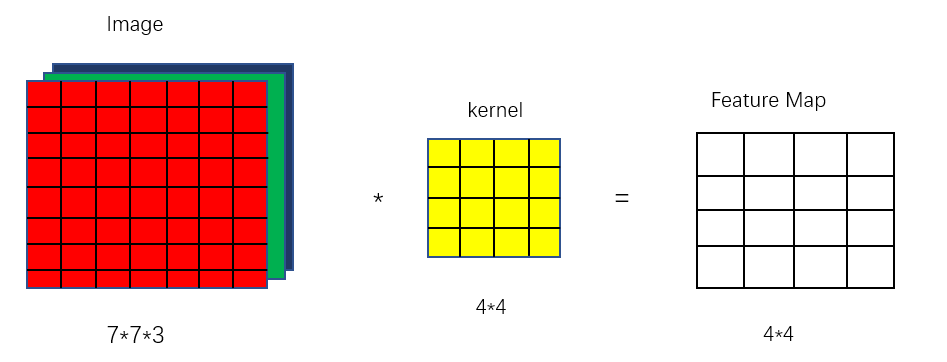
\includegraphics[width=0.95 \textwidth,clip]{conv.png}
	%\hspace{0.02\textwidth}
	%\vspace*{-0.08cm}
    \caption{卷积神经网络的卷积层示意图}
	\vspace*{-3.5mm}
	\label{fig:conv-example}
\end{figure}


\subsubsection{经典的卷积神经网络结构}





\subsection{物体检测与识别}

在社会关系识别的任务中,有一个重要的模块是利用物体识别模型得到人的场景信息,即采用物体识别模型识别去当前图片中包含了哪些物体,得到该物体在图片的区域。物体识别的模型包括Ross等人提出的RCNN\cite{DBLP:conf/cvpr/GirshickDDM14},fast-RCNN\cite{DBLP:conf/iccv/Girshick15},以及Ren等人(2016)\cite{DBLP:conf/nips/RenHGS15}提出的faster-RCNN。前面提到的三个模型都是基于区域的物体检测模型,RCNN\cite{DBLP:conf/cvpr/GirshickDDM14}首次提出在目标图像中有多个目标框,然后判断目标框是否包含物体,具体的检测步骤如下:
(1)其中采用选择性搜索的方法得到图片中的所需要的目标框区域,将得到的区域调整为卷积神经网络输入的消息。
(2)利用一个预训练好的卷积神经网络,提取第一步得到的区域中的特征。
(3)将第二步中得到的特征当作一个线性SVM的输入,得到物体的类别,另外训练一个线性回归模型得到物体的目标框。
RCNN的主要缺点是对于一张图片中的每个感兴趣区域,需要遍历提取其中的特征,然后依次执行物体的分类和物体框的回归,需要耗费较多时间。由于全卷积和池化层不改变某个区域在特征图和原图的位置,因此fast-RCNN 在RCNN 的基础上提出了ROI(region of interest) 池化层,将图片输入到卷积神经网络中,对于特征图上的区域,经过ROI池化层进行调整,然后再继续之后的全连接层和一个线性回归层进行分类和目标框的确定。综上,fast-RCNN 较大程度上提高了物体检测的性能。由于fast-RCNN 在大数据集上的表现依然不能满足实际的需求,因为RCNN和fast-RCNN均采用选择性搜索的方法得到所需要的区域,这个步骤是比较耗费时间。因此faster-RCNN提出RPN(region proposal network),RPN主要网络包括两部分,一部分主要是对生成的anchors进行判断是foreground还是background,其中foreground代表目标,另外一部分主要是对检测框的位置进行调整。经过RPN网络后得到候选区域,再利用ROI池化得到特征向量进行物体类别的判断和物体框的进一步精确判断。

综上,以上的篇幅主要是回顾了在社会关系检测的工作中,有用的物体检测方法和一些相关工作。结论是得益于GPU等硬件设备的发展,物体识别领域的算法也得到了快速的发展,尤其是随着特征提取模块的发展,卷积网络越来越深,能学习到更多更丰富的特征。对于一幅图片,我们能在得到更多的、更准确的物体框和类别。

\section{社会关系检测}
本章将回顾社会关系检测领域的一些相关工作,并且对于消息传递机制的介绍,以及消息传递机制的相关工作的一些介绍。

\subsection{已有工作的简单介绍}

社会关系检测是社交网络的一个基础,社会关系检测作为一个重要的多学科问题,在计算机视觉领域受到越来越多的关注。随着这个问题被提出以来,有大量的工作用于从图片中抽取两个人之间的社会关系。主要有Zhang等人(2015)\cite{DBLP:conf/iccv/ZhangLLT15}提出的利用面部表情、年龄、性别、姿势等多种特征的联合模型。Li等人(2017)\cite{DBLP:conf/iccv/LiWZK17}提出的多次观察的Dual-glance模型。以及Wang等人(2018)\cite{DBLP:conf/ijcai/WangCRYCL18}提出的基于常识知识的深度推理模型GRM。

Zhang等人提出的模型认为从心理学的角度出发,认为人的关系主要由人的面部表情的一些特点决定的。首先,模型设计了一个基准模型用于提取图片中两个人对的特征,对于两个人对,基准模型采用共享参数的深度卷积网络(DCN),利用DCN提取得到的特征分别记为$x^r,x^l$,并且$\forall x^r,x^l \in R^{2048 \times 1}$,经过一个权重矩阵$\mathbf{W} \in R^{4096 \times 256}$得到特征向量$x_t$。对于已经标注好的人脸图片两个人脸分别为和,利用DCN 提取得到的特征分别记为和,并且。除了图片中本来的特征,模型利用了两张人脸在图片的空间信息。1)两张人脸的位置分别表示为${x^l,y^l,w^l,h^l,x^r,y^r,w^r,h^r}$,其中$x-,y-$是左上角的坐标,$w,h$ 分别是两个人脸包围盒的宽度和高度。2)人脸的相对位置$\frac{x^l-x^r}{w^l},\frac{y^l-y^r}{h^l}$。3)人脸之间的比例$\frac{w^l}{w^r}$。以上的三项空间特征会和DCN得到的$x_t$拼接来学习得到关系类别。
\begin{figure}[htpb]
	\centering
	%	\includegraphics[width=0.48 \textwidth, trim=10 10 10 80,clip]{./pic/example_new.pdf}
	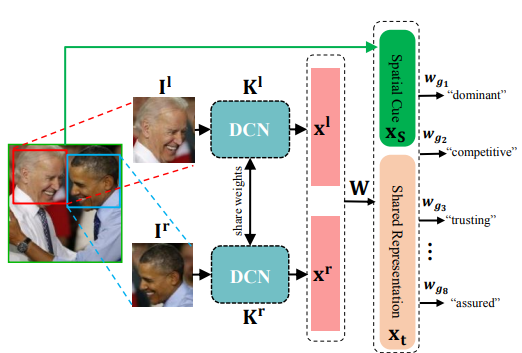
\includegraphics[width=0.75 \textwidth,clip]{1.png}
	%\hspace{0.02\textwidth}
	%\vspace*{-0.08cm}
    \caption{zhang的模型}
	\vspace*{-3.5mm}
	\label{fig:model_zhang}
\end{figure}
\looseness=-1
除此之外,$\mathbf{w_{gi}}$,$\mathbf{W}$,$\mathbf{K^l}$,and $\mathbf{K^r}$可以采用标准的正太分布初始化。结合之前符号的定义,该模型损失函数定义如下:
\begin{equation}
\begin{split}
     arg\max \limits_{\Omega} p({\mathbf{w}_{g_i}}_{i=1}^8, \mathbf{W},\mathbf{K}^r | \mathbf{g},\mathbf{x}_t,\mathbf{x}_s,\mathbf{I}^r,\mathbf{I}^l) \propto \\
     (\sum_{i=1}^{8}p(g_i|x_t,x_s)p(w_(g_i)))(\sum_{j=1}{K}p(k_j^l)p(k_j^r))p(\mathbf(W)), \\
     s.t. \mathbf{K}^r = \mathbf{K}^l
\end{split}
\end{equation}
基于以上的工作,该模型同样认为人的面部属性对最终的关系预测可以起到关键的作用。

Li等人\cite{DBLP:conf/iccv/LiWZK17}在前面的工作,针对社会检测的任务提出了包含两个关系粒度的数据集,PISC\cite{DBLP:conf/iccv/LiWZK17}。该工作首次提出了利用图片中的场景来协助预测两个人之间的关系,场景具体表示为该图片中的物体。直观来说,如果一幅图片中包含电脑桌子等物体,那么大概率是``同事''关系。模型分为两个模块,first glance和second glance,first glance的输入为一张图片$\mathbf{I}$ 和两个人身体的包围盒。针对图片$I$,首先修剪出3个小块,前两个小块分别覆盖住两个人,$p_1$和$p_2$,第三个小块覆盖两个人,表示为$p_{u}$。这三个小块的像素被修正为$224 \times 224$大小,作为后续三个CNNs 网络的输入

